\chapter{Dataset}
\label{ch:dataset}
 
%
% Section: 4 - Intro
%

Training and evaluation of automatic information extraction approaches requires availability of reliable ground truth data of sufficient size. Following a growth of interest for extraction of information about software tools from scientific publications labeled data sets with limited scope such as BioNerDs, SoftCite, SoSciSoSci have came into existence. More recently, \ac{SoMeSci} data set, a more comprehensive corpus that covers a wide range of information about software tools has also been introduced \citep{schindler2021somesci}.  \\

This section describes the data set used in this project – \ac{SoMeSci},  the extension process with software usage purpose annotations, issues observed during annotation, pre-processing of the data-set, analysis results of the data and transformation to a suitable format for training purpose.  


\section{SoMeSci dataset}
\label{sec:dataset:SoMeSci}

\ac{SoMeSci} data set contains high quality, hand annotated articles collated from  \ac{PMC}. The articles and annotations included in the data set are summarized below.  

\subsection{ SoMeSci Articles }
\label{subsec:dataset:SoMeSci:Articles}

The corpus is composed of four group of files, namely\emph{PLoS methods, PLoS sentences, PubMed full text} and \emph{Creation sentences}. Facts about the articles in the \ac{SoMeSci} corpus is summarized in the table 4.1. \\

\begin{table}
	\caption{Article composition of  \ac{SoMeSci} dataset.}
	\begin{tabularx}{\textwidth}
		{|>{\setlength\hsize{.6\hsize}\setlength\linewidth{\hsize}}X|>{\setlength\hsize{1.4\hsize}\setlength\linewidth{\hsize}}X|}
		
		\hline
		SoMeSci article & Description  \\
		\hline
		1. PLoS Methods   &
		- 480 articles from PLoS journal that contain only methods sections\\
		\hline
		2. PubMed full text   &
		- 100 randomly selected full-articles from PMC Open Access\\
		\hline
		3. PLoS sentences  &
		- 677 files extracted from PLoS articles which contain sentences that has software names mentioned in them.  \\
		\hline
		4. Creation sentences  &
		- 110 files that contain sentences indicating creation of a software  files out of which 50 are extracted from PMC OA, where as the rest 60 are from PLoS.  \\
		\hline
		
		\emph{Total} &
		- 1367 files  \\
		\hline

	\end{tabularx}
\end{table}

\subsection{SoMeSci Annotations  }
\label{subsec:dataset:SoMeSci:Annotations }

SoMeSci corpus has three main types of annotations that correspond to a type of information related with software tools. These annotations indicate the type of software, type of mention and additional information about the software as summarized on the table 4.2. \\ 

\begin{table}
	\caption{Annotation composition of \ac{SoMeSci} dataset before its extension with software usage purpose labels.}
	\begin{tabularx}{\textwidth}
		{|>{\setlength\hsize{.6\hsize}\setlength\linewidth{\hsize}}X|>{\setlength\hsize{1.4\hsize}\setlength\linewidth{\hsize}}X|}
		
		\hline
		Annotation category & Types of Annotations  \\
		\hline
		4 software-types   &
		- Application , Plugin , Operating System and Programming Environment\\
		\hline
		4 mention types  &
		- Mention, Usage, Creation, and Deposition\\
		\hline
		9 additional info.  &
		- Developer, Version, \ac{URL}, Extension, Release, License, Abbreviation, \& Alternative name.\\
		\hline
		
	\end{tabularx}
\end{table}

\section{Annotation tool}
\label{sec:dataset:tool}
The data set has been annotated using BRAT rapid annotation tool (version 1.3) (\href{https://scicrunch.org/resolver/SCR_008769}{RRID:SCR\_008769})  in a Linux 20.4 environment. The annotation tool has been run in a local machine as a \ac{CGI} application using a browser. 

\begin{figure}[htbp]
	\centering
	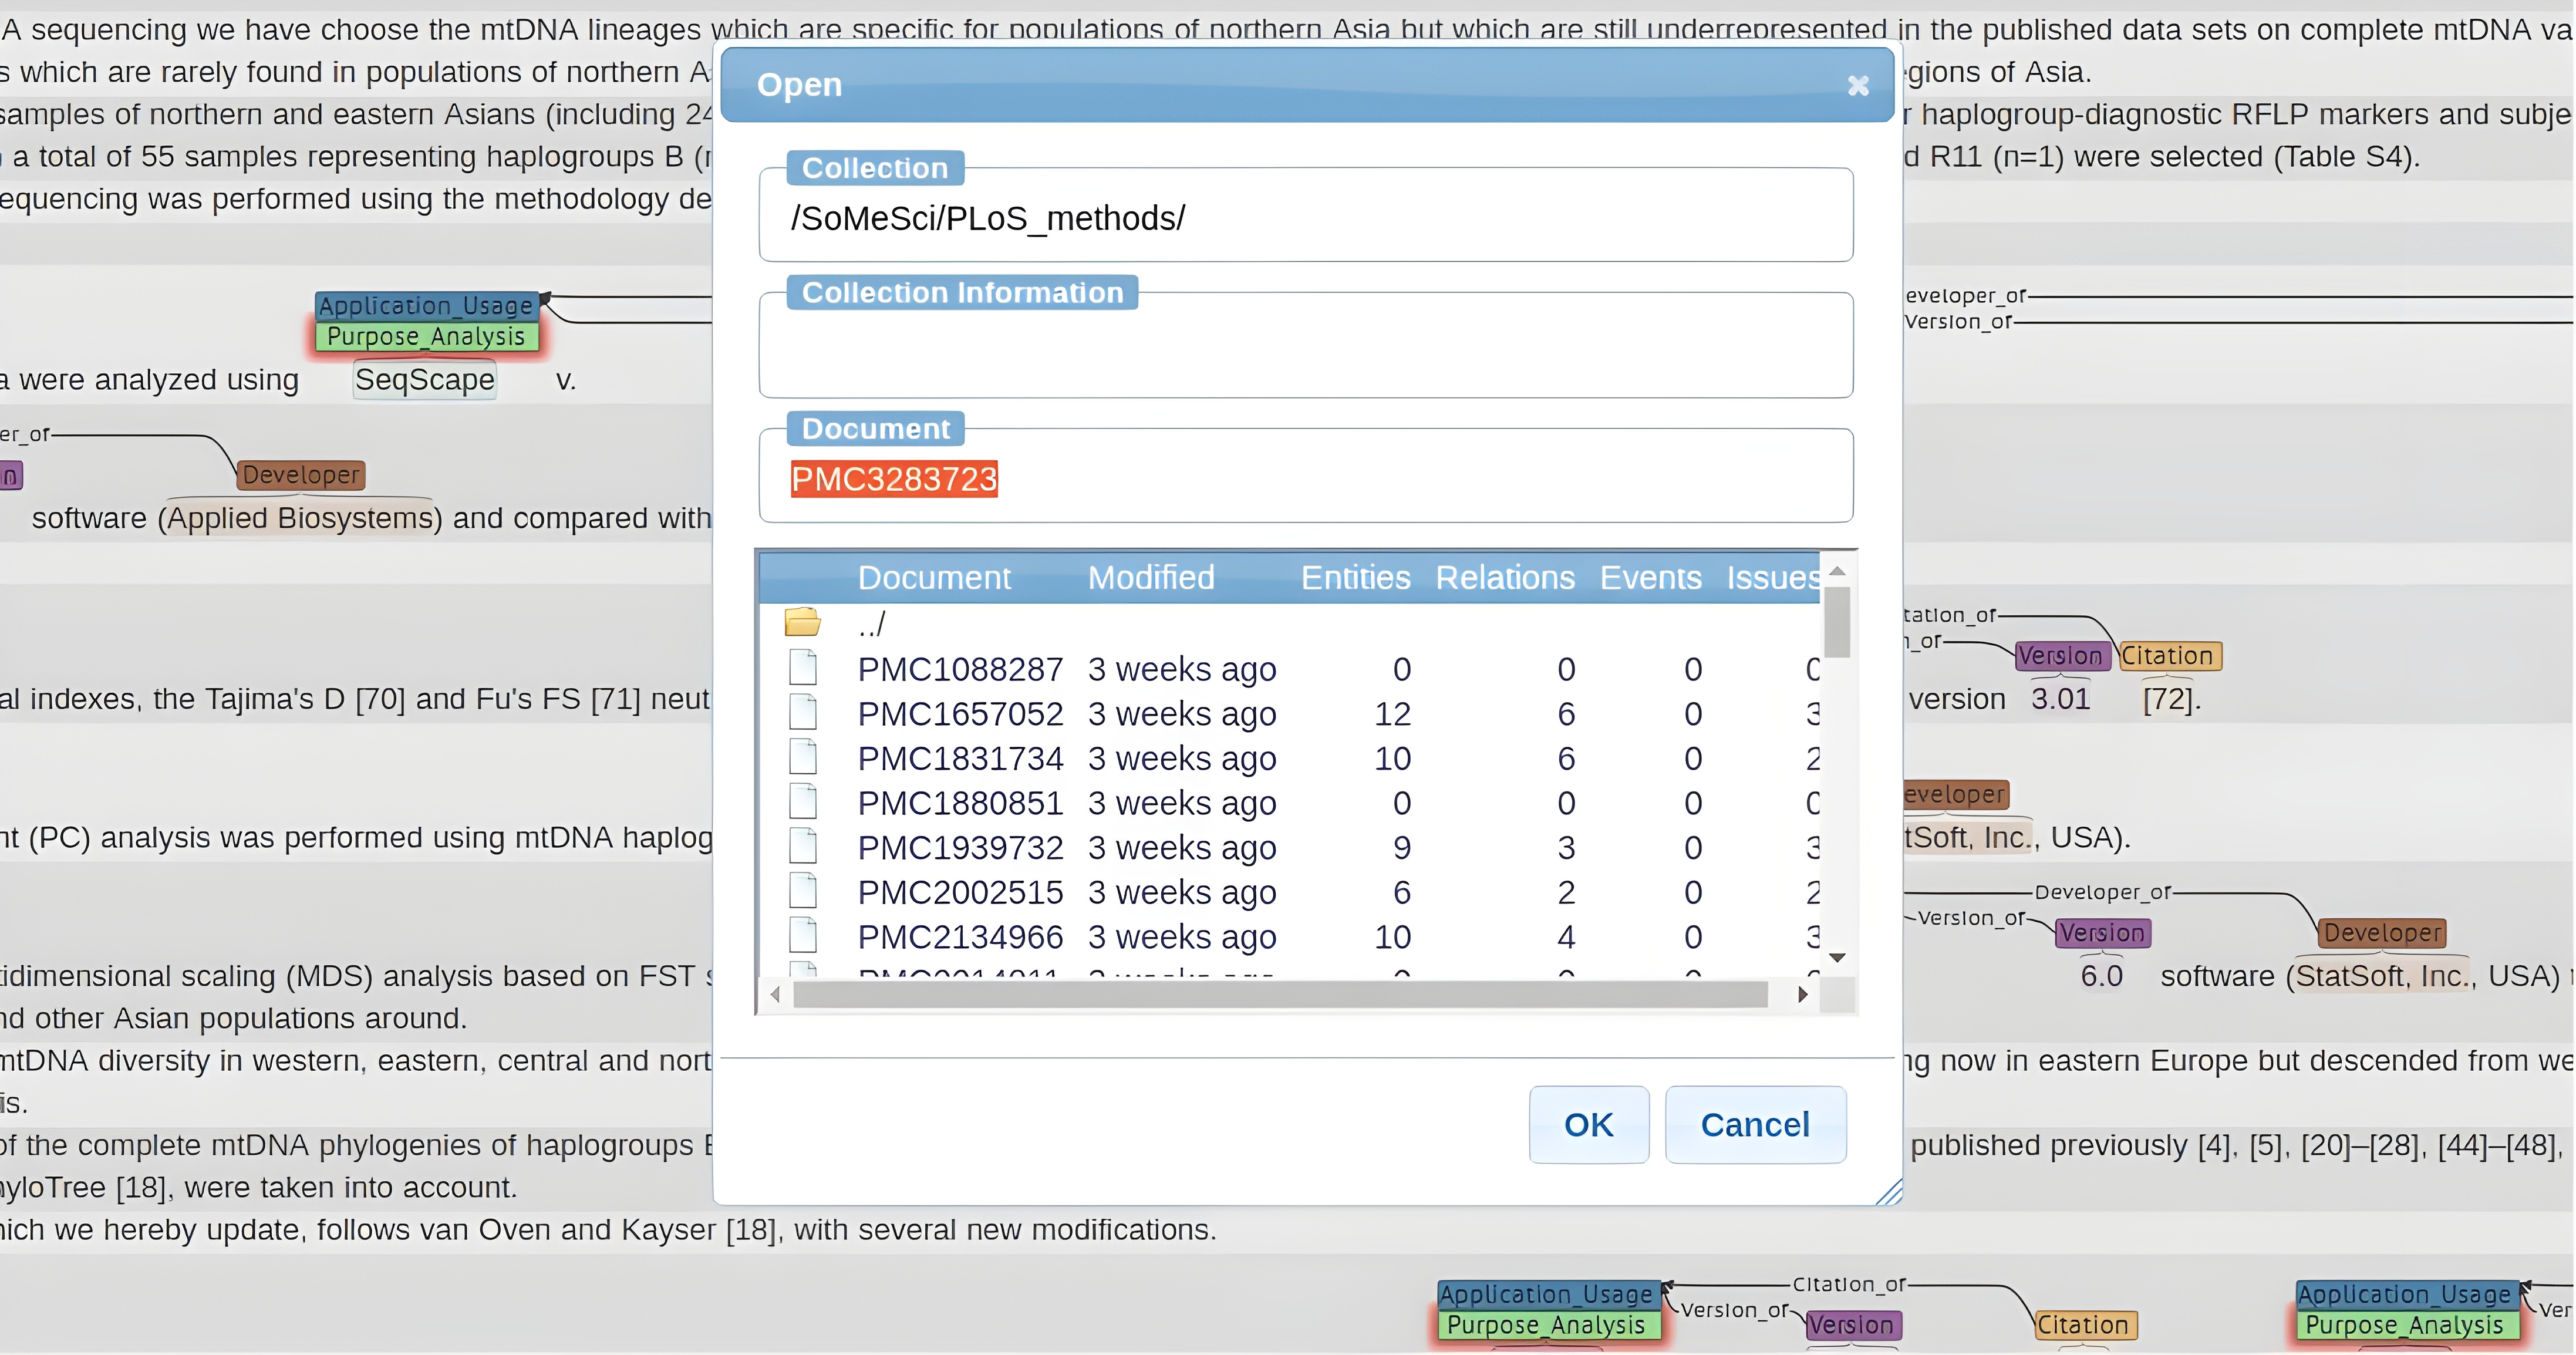
\includegraphics[width=.66\textwidth]{4.graphics/figures/ch_4/BRAT_tool}
	\caption{BRAT annotation tool}
	\label{fig:chapter04:setup}
\end{figure}

\subsection{Annotation of SoMeSci with software purpose labels}
\label{subsec:dataset:tool:Annotationprocess}

\ac{SoMeSci} corpus has been extended with annotations of eight classes of purpose of software usage labels  identified in the earlier section (summarized in table 3.7). Since using software for a particular purpose only refers to the usage of a software, only usage annotations among the 4 types of annotations described in the table 4.2), have been further labeled with software purpose. The figures below show \ac{SoMeSci} data set before and after software purpose annotations. \\

\begin{figure}[htbp]
	\centering
	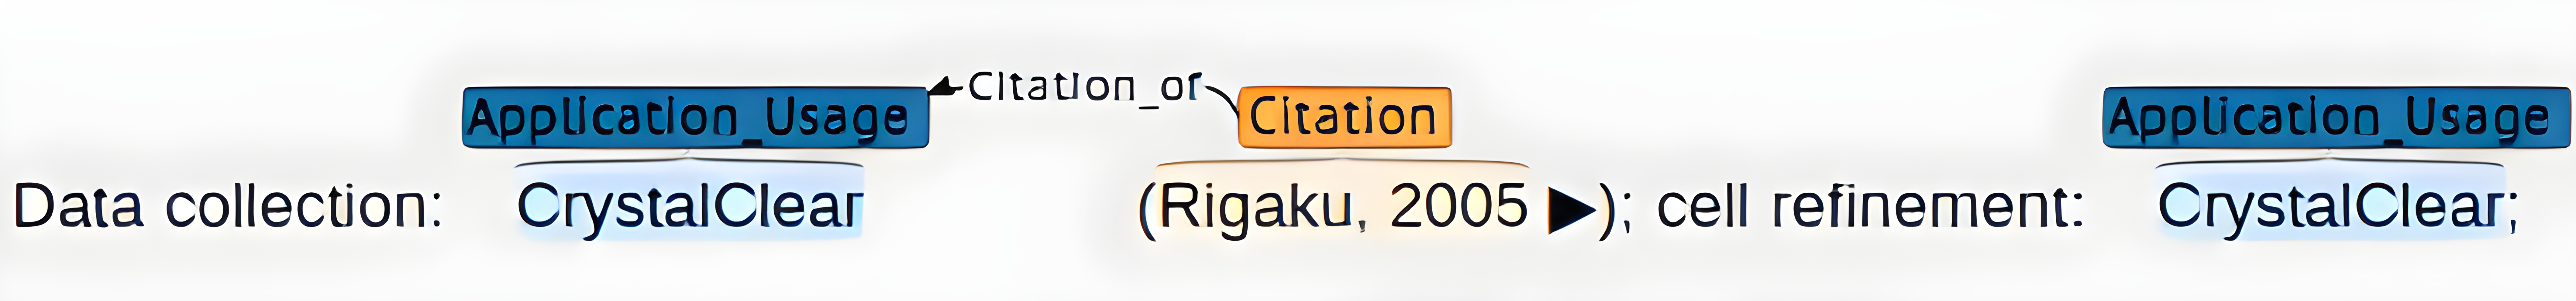
\includegraphics[width=.85\textwidth]{4.graphics/figures/ch_4/before_ann_hd_PMC3120364_FULLTEX_HD}
	\caption{Original annotations in \ac{SoMeSci} dataset before extension with software usage purpose annotations }
	\label{fig:chapter04:setup}
\end{figure}

\begin{figure}[htbp]
	\centering
	
\includegraphics[width=.85\textwidth]{4.graphics/figures/ch_4/after_ann_hd}
	\caption{\ac{SoMeSci} annotations after extension with software usage purpose labels}
	\label{fig:chapter04:setup}
\end{figure}


\subsection{Top-level annotation}
\label{subsec:dataset:tool:Assumptions}

For the sake of simplicity, certain types of software usages have been assigned the same class of software purpose annotation. For example, modeling might refer to graphical modeling of an object using \ac{CAD} software or it might also refer to mathematical representation of a given problem.  All such variants of modeling tasks have been assigned “modeling” , a top-level class, as a label without differentiating specific variants. 


\subsection{Challenges during Annotation }
\label{subsec:dataset:tool:Challenges}

There were cases where a given software had multiple types of software usage purpose where throughout the annotation process only a single software usage purpose was being assigned. In such cases,  annotations has been carried out in a such way by deciding on each context which software purpose annotation is more important or based on the general goal of the software usage. \\

For example, FlexArray software on the figure below, has been annotated with software purpose analysis even though the same software was used for visualization purpose as well. This is because on this context analysis is more important than visualization and essentially visualization could also be interpreted as one kind of analysis. In addition, specific definition of each of software usage purposes has been also taken into account. \\

\begin{figure}[htbp]
	\centering
	\includegraphics[width=.99\textwidth]{4.graphics/figures/ch_4/Ann_confusion_HD}
	\caption{Selection of priority for annotations based on context: Visualization is one form of analysis hence label analysis is selected over visualization }
	\label{fig:chapter04:setup}
\end{figure}

However, in some instances, annotation of software-purposes appears to be ambiguous. For example a software used for counting or quantification can be assigned a software purpose label of  \emph{data collection} but also \emph{analysis}. Such cases of annotation with software usage purpose are subjective and can affect the over all annotation quality.\\

The other challenge of annotation was difficulty arising from limited domain knowledge. In some cases, labeling of purpose of use of a software was quite difficult because of lack of understanding what the scientists were trying to do using the software.

\section{Data Pre-processing}
\label{sec:dataset:preprocessing}
Pre-processing of the data set has been carried out to ensure the integrity of our data set before using it in the classifier. The data pre-processing tasks handled annotation errors, merging annotations , transforming and splitting of data set. 

\subsection{Automatic Integrity Testing }
\label{subsec:dataset:preprocessing:handlingerrors}

As described in the above table, the four types of software mentions in the SoMeSci are mention, usage, creation and deposition. The main goal of annotating the data set was to assign corresponding purpose of software usage label to each instance of software usage but not for mention, creation and deposition. However, due to an error there were some instances of software mention that has been annotated with software purpose. In addition to this, there were also some instances of usage, that has not been annotated and intentionally skipped because of the purpose of software usage did not seem to be clear. \\

Therefore, all instances of wrong or missing annotations have been identified automatically to ensure the integrity of training data set.The python code for automatic identification of annotation errors has been listed under \emph{Appendix-B}.

\subsection{Merging Annotations}
\label{subsec:dataset:preprocessing:Merging}

After handing all annotation errors and missing labels, annotations of software usage has been merged with annotations of software purpose. Merging of the annotations has been carried out to unify and integrate software usage purpose annotations with the original annotations. The python code for merging annotations has been listed on the \emph{Appendix-C}. Figures 4.5 and 4.6 below shows, software purpose labels before and after integration into the original annotation respectively.  \\

\begin{figure}[htbp]
	\centering
	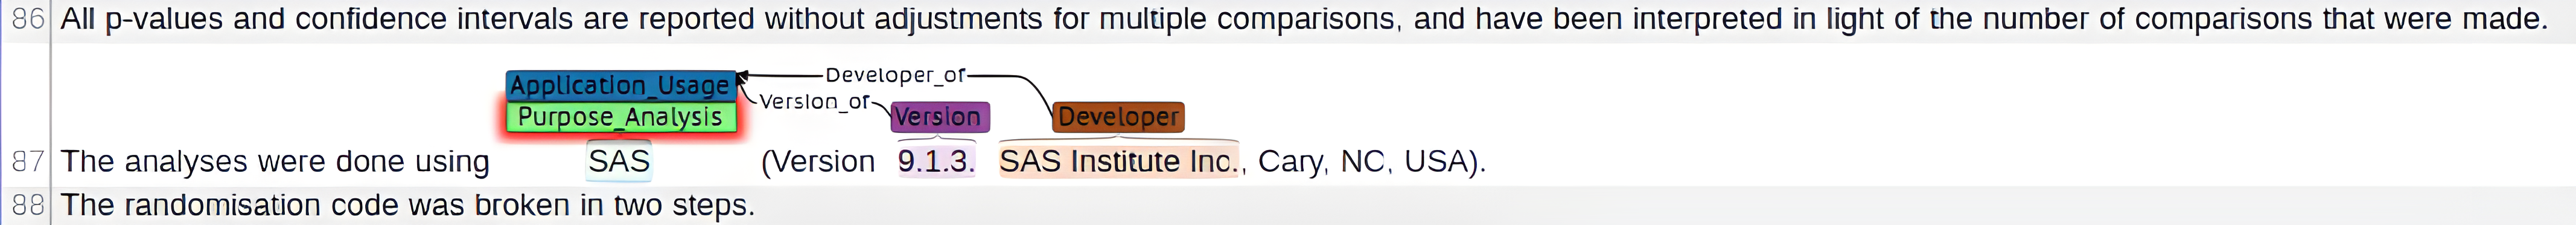
\includegraphics[width=.75\textwidth]{4.graphics/figures/ch_4/2002515_plm_unm_HD}
	\caption{Software usage annotations before merging with software purpose  annotation.}
	
	\label{fig:chapter04:setup}
\end{figure}

\begin{figure}[htbp]
	\centering
	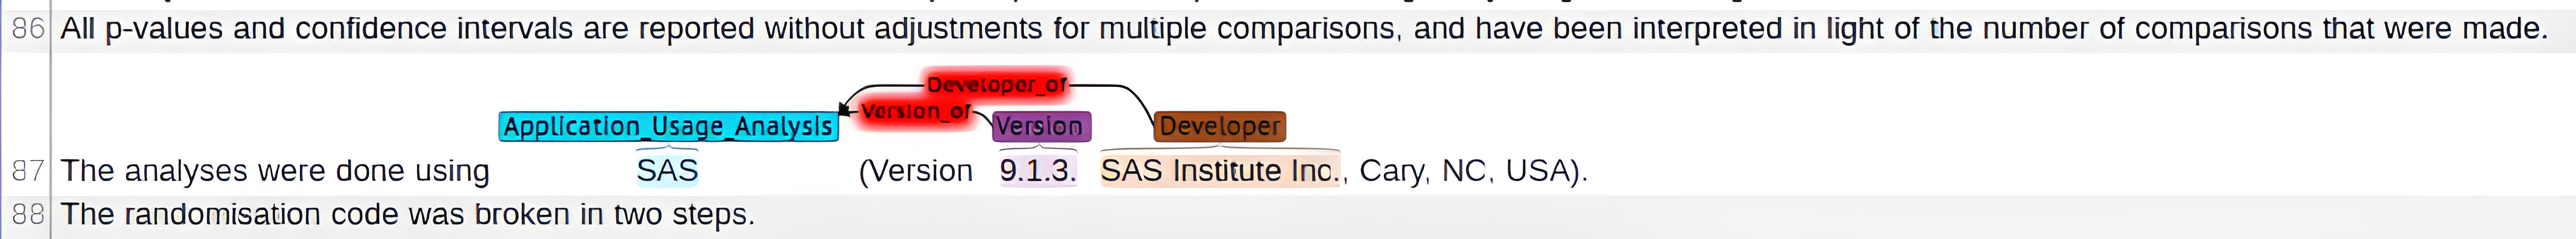
\includegraphics[width=.75\textwidth]{4.graphics/figures/ch_4/2002515_plm_HD}
	\caption{Software usage annotations after merging with software purpose  annotation.}
	\label{fig:chapter04:setup}
\end{figure}


\subsection{Transformation to IOB format}
\label{subsec:dataset:preprocessing:Transformation}
After merging software usage and purpose labels, transformation of data into IOB format has been carried out using articlenizer (link to articlenizer). Figure 4.7 below shows the data format before and after transformation. \\

\begin{figure}[h]
	
	\myfloatalign
	
	\subfloat{
		\label{fig:chapter03:subfloat:grafik1}
		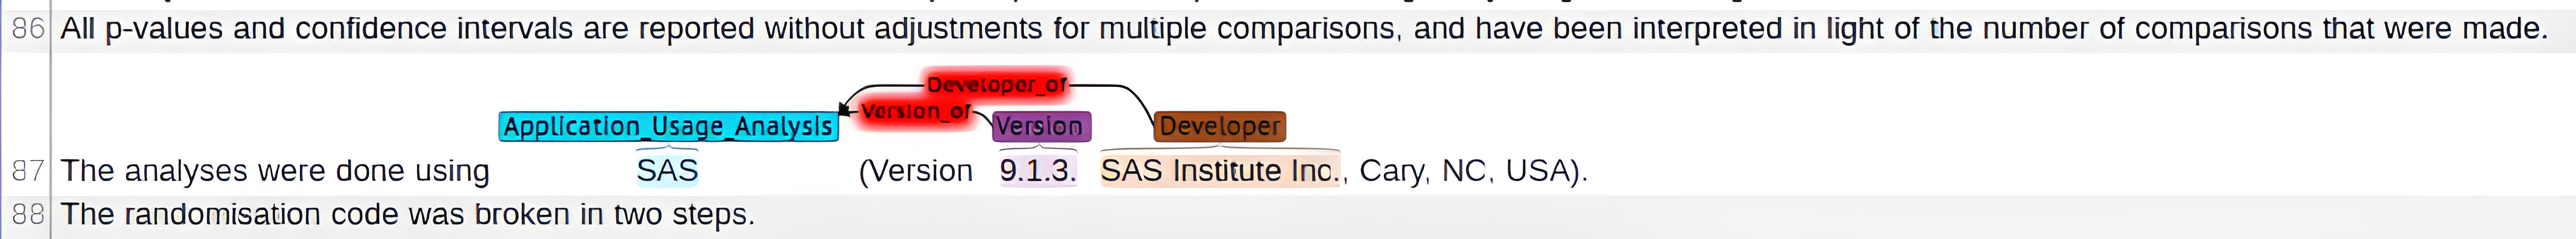
\includegraphics[width=.98\linewidth]{4.graphics/figures/ch_4/2002515_plm_HD}
	} \\
	\subfloat{
		\label{fig:chapter03:subfloat:grafik4}
		
\includegraphics[width=1\linewidth]{4.graphics/figures/ch_4/BIo_2002515_plosmet_HD}
	}\\
	\caption{Merged software usage and purpose annotation \& its corresponding IOB representation.}
\end{figure}




\section{Analysis of Annotated Data}
\label{sec:dataset:Analysis}

Analysis of cleaned SoMeSci data set has been carried out to find a deeper insight about the training data. 

\subsection{Co-reference resolution of software entities }
\label{subsec:dataset:Analysis:resolution}

The base line for the analysis of the data set was to carry out disambiguation of software names. This was particularly important because there is large degree of variation in software names. Using list of software name with corresponding URL, software mention instances have been disambiguated from each other and all software name variations that refer to the same entity have been given the same name. \\

Figure 4.8 below shows name variations for MATLAB software, in which all instances resolve to the same URL i.e. entities referring to the same software. All variations of names has been replaced by the first “Matlab” in this case.

\begin{figure}[htbp]
	\centering
	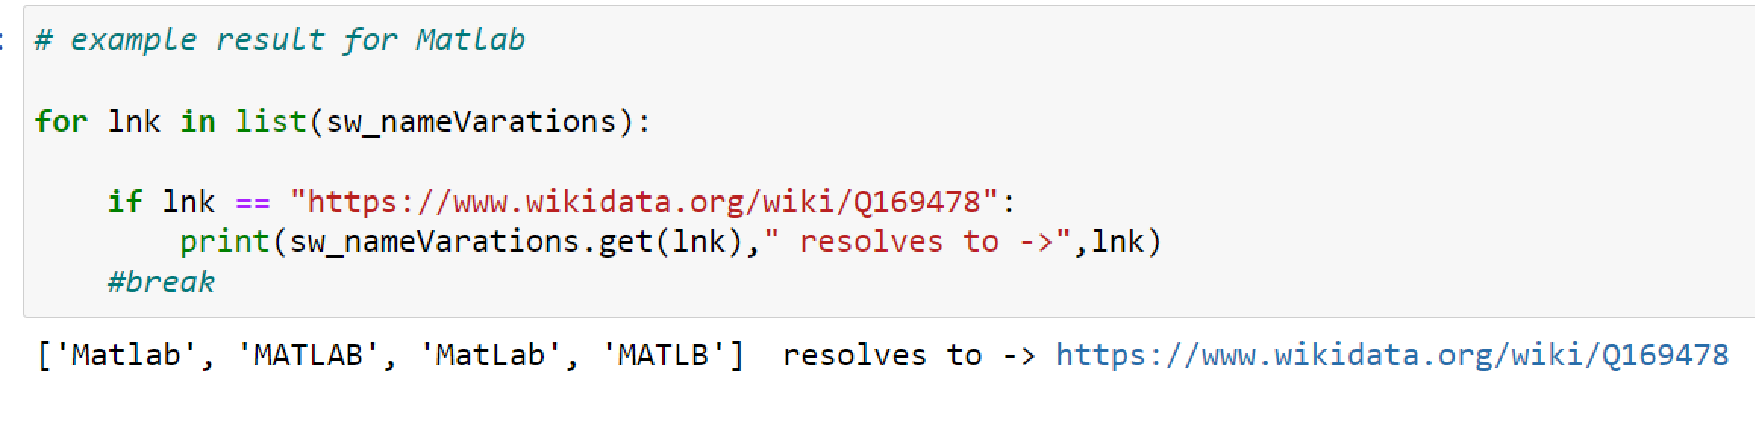
\includegraphics[width=1\textwidth]{4.graphics/figures/ch_4/pdf/Corefresolution}
	\caption{Example of Co-reference resolution for Matlab software. All name variations have been given the same name.}
	\label{fig:chapter04:setup}
\end{figure}


\subsection{Analysis results }
\label{subsec:dataset:Analysis:results}

According to the analysis results, the top 3 software by number of software name mention count through out the list of articles in PubMed and PLoS data set are: PASW, GNU-R and STATA as shown on the figure 4.9 below. 

\begin{figure}[htbp]
	\centering
	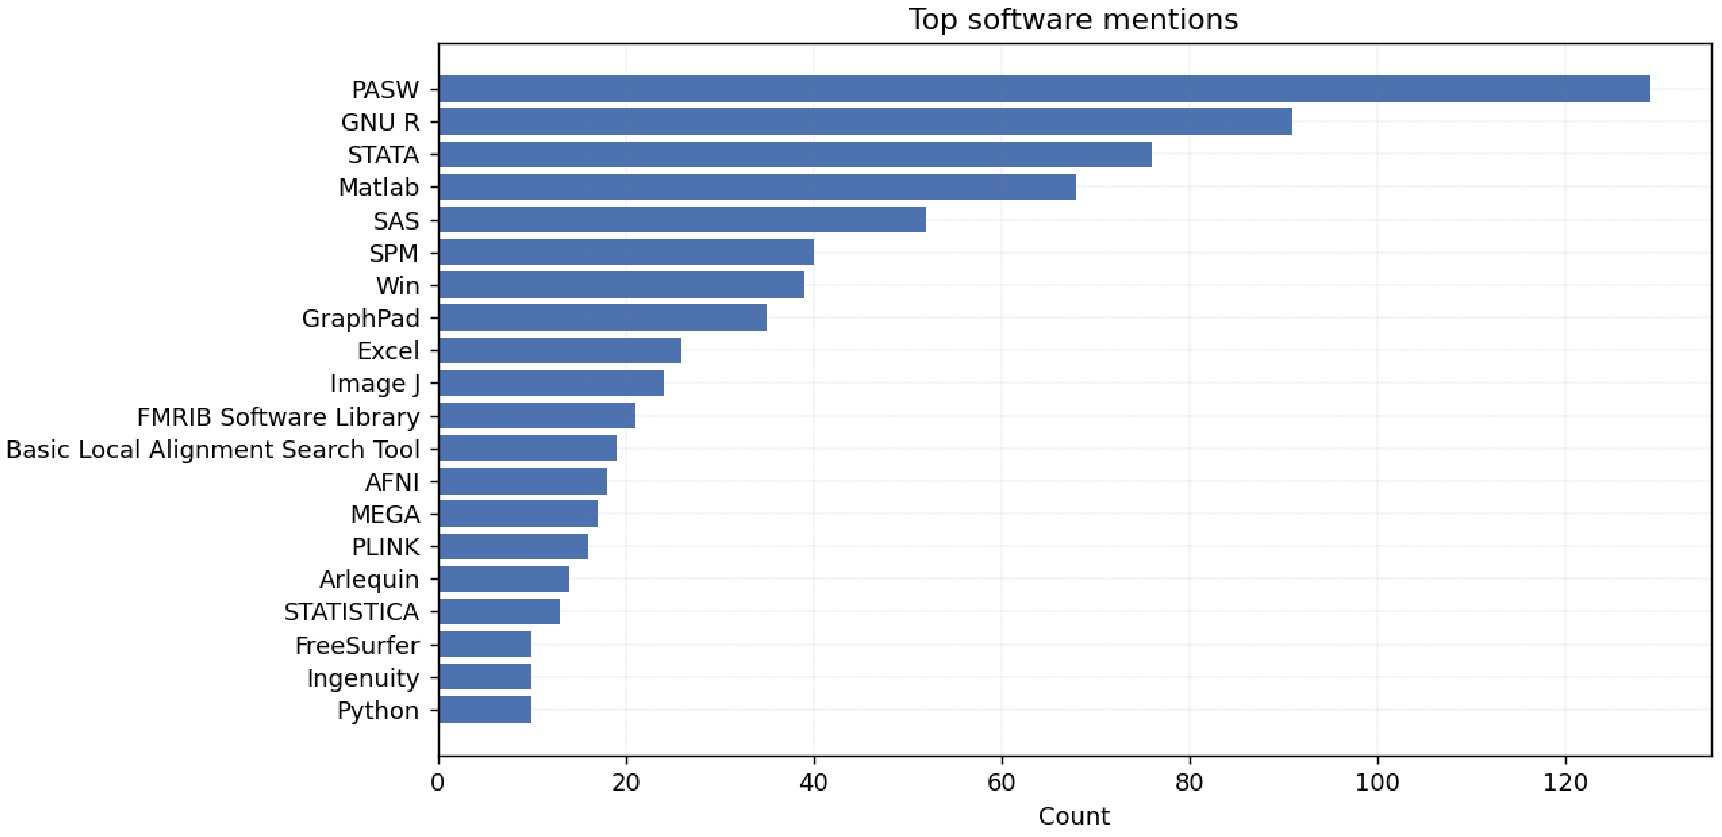
\includegraphics[width=.90\textwidth]{4.graphics/figures/ch_4/analysisresults/1.Top software mentions}
	\caption{Top software mentions}
	\label{fig:chapter03:setup}
\end{figure}

Data set analysis result from the perspective of purpose of software usage indicates that the most common purpose of software usage are: Analysis, Data pre-processing, Data collection and modeling where as the least common are simulation and stimulation. The result is shown on figure 4.10 below. \\

The other insight form from  the software-type perspective, is that the most commonly used type of software in the research articles in the data set is Application software as depicted on figure 4.11. \\

\begin{figure}[h]
	\myfloatalign
	\subfloat[software purpose]{
		\label{fig:chapter03:subfloat:grafik1}
		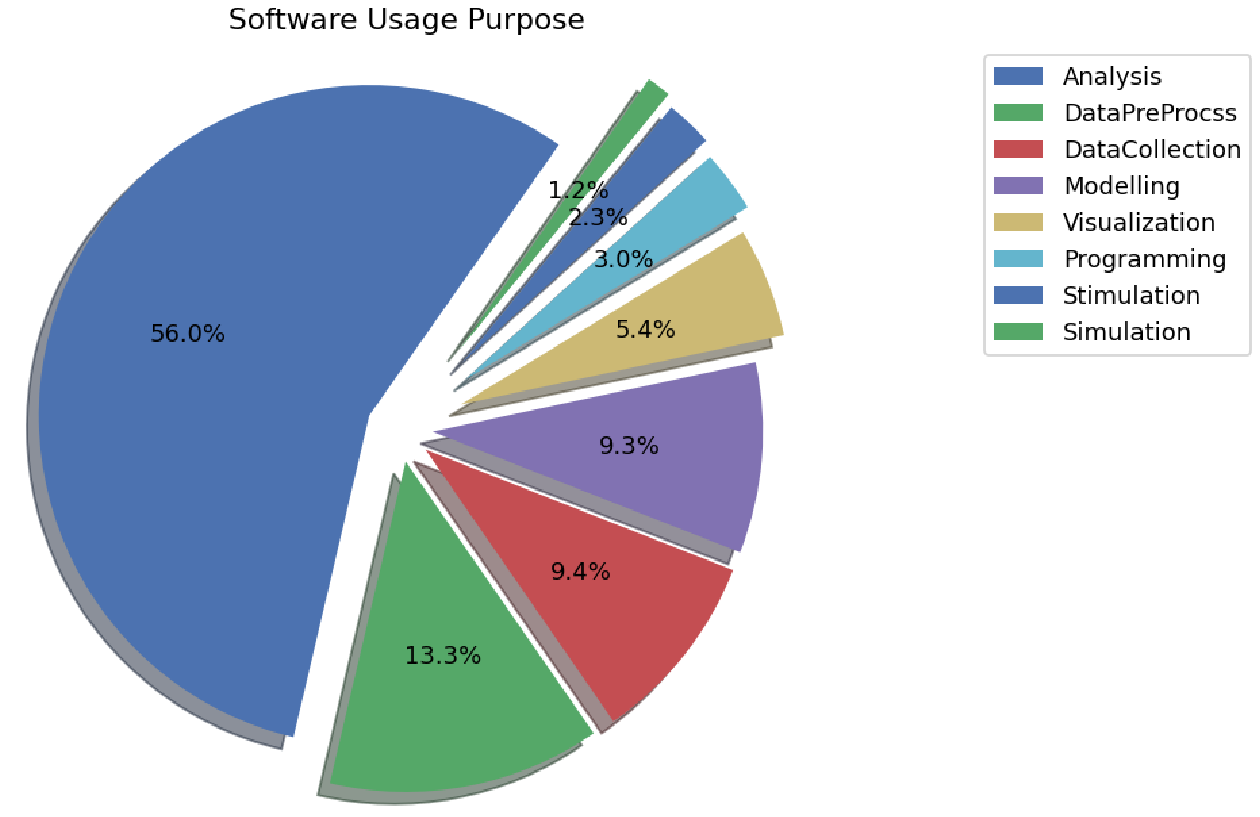
\includegraphics[width=.47\linewidth]{4.graphics/figures/ch_4/analysisresults/2.Software Usage Purpose pie}
	} \quad
	\subfloat[Types of software] {
		\label{fig:chapter03:subfloat:grafik2}
		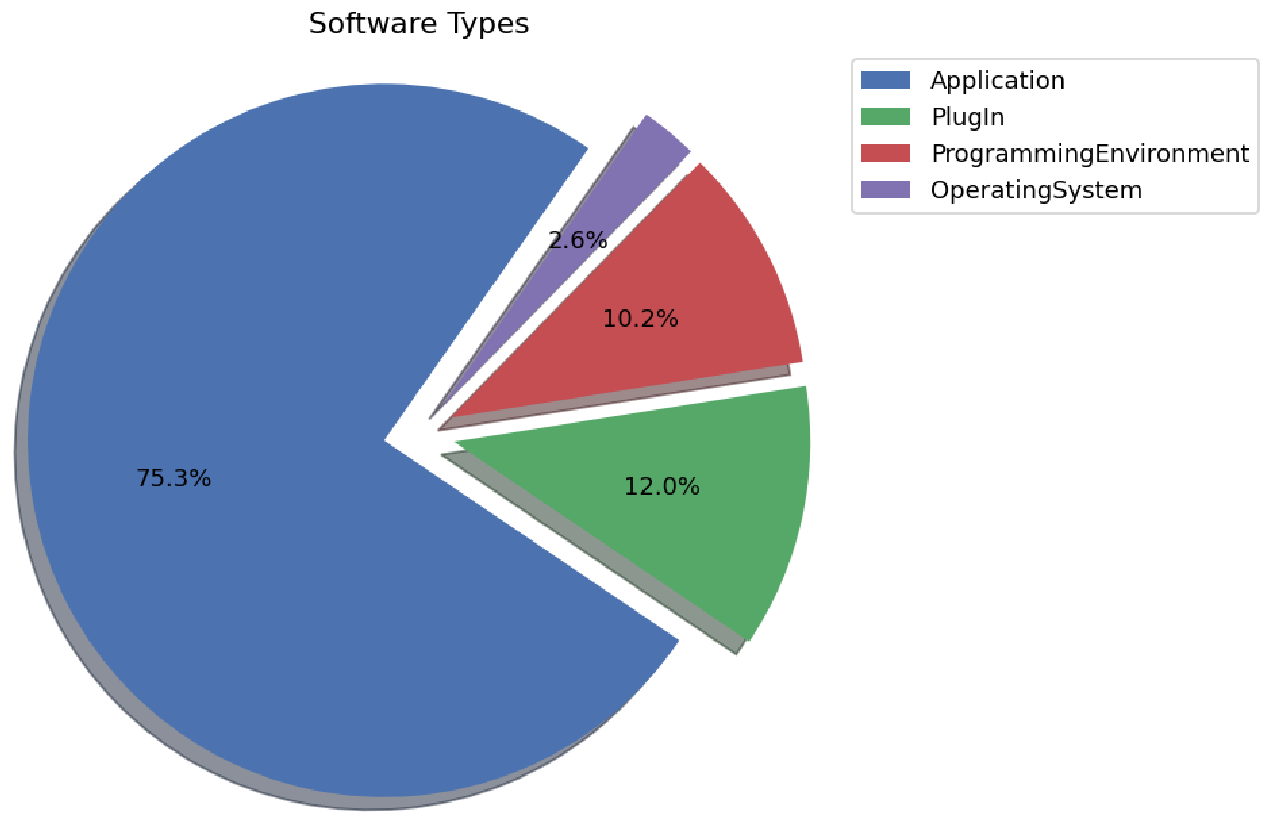
\includegraphics[width=.47\linewidth]{4.graphics/figures/ch_4/analysisresults/4.Software Types pie}
	} \\
	\caption{Software usage purposes and types of software in the SoMeSci data set.}
	
\end{figure}


When it comes to share of each purpose of software usage among the 4 types of software, the pattern once again clearly indicates most of the time a software has been used for the purpose of analysis and data collection in all of the four software types. \\

\begin{figure}[htbp]
	\centering
	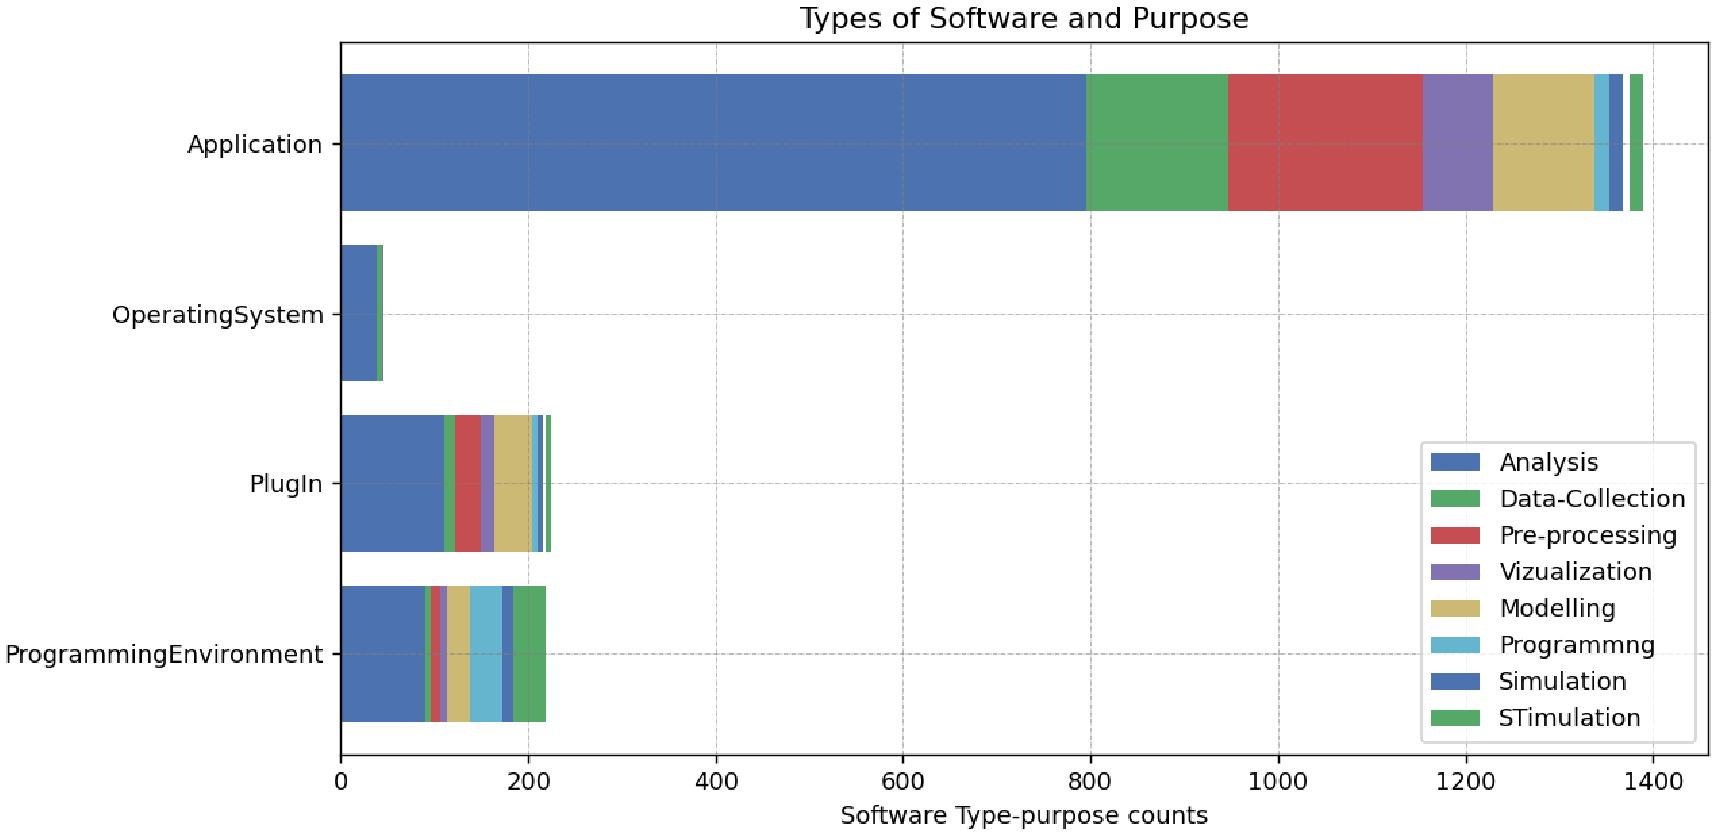
\includegraphics[width=.90\textwidth]{4.graphics/figures/ch_4/analysisresults/6.Types of Software and Purpose stacked bar}
	\caption{Share of software usage purpose from each type of software in the \ac{SoMeSci} data set.}
	\label{fig:chapter03:setup}
\end{figure}

Lastly, the other interesting insight observed from analysis of the data set was determining: ” For how many different purposes has a given software been used ?”.  The analysis reveals that from 657 unique software, nearly 76\% have been used only for a single purpose as shown on the bar graph 4.12 below. Over all, this result indicates that most of the time software tools have been used only for a specific purposes.


\begin{figure}[h]
	\centering
	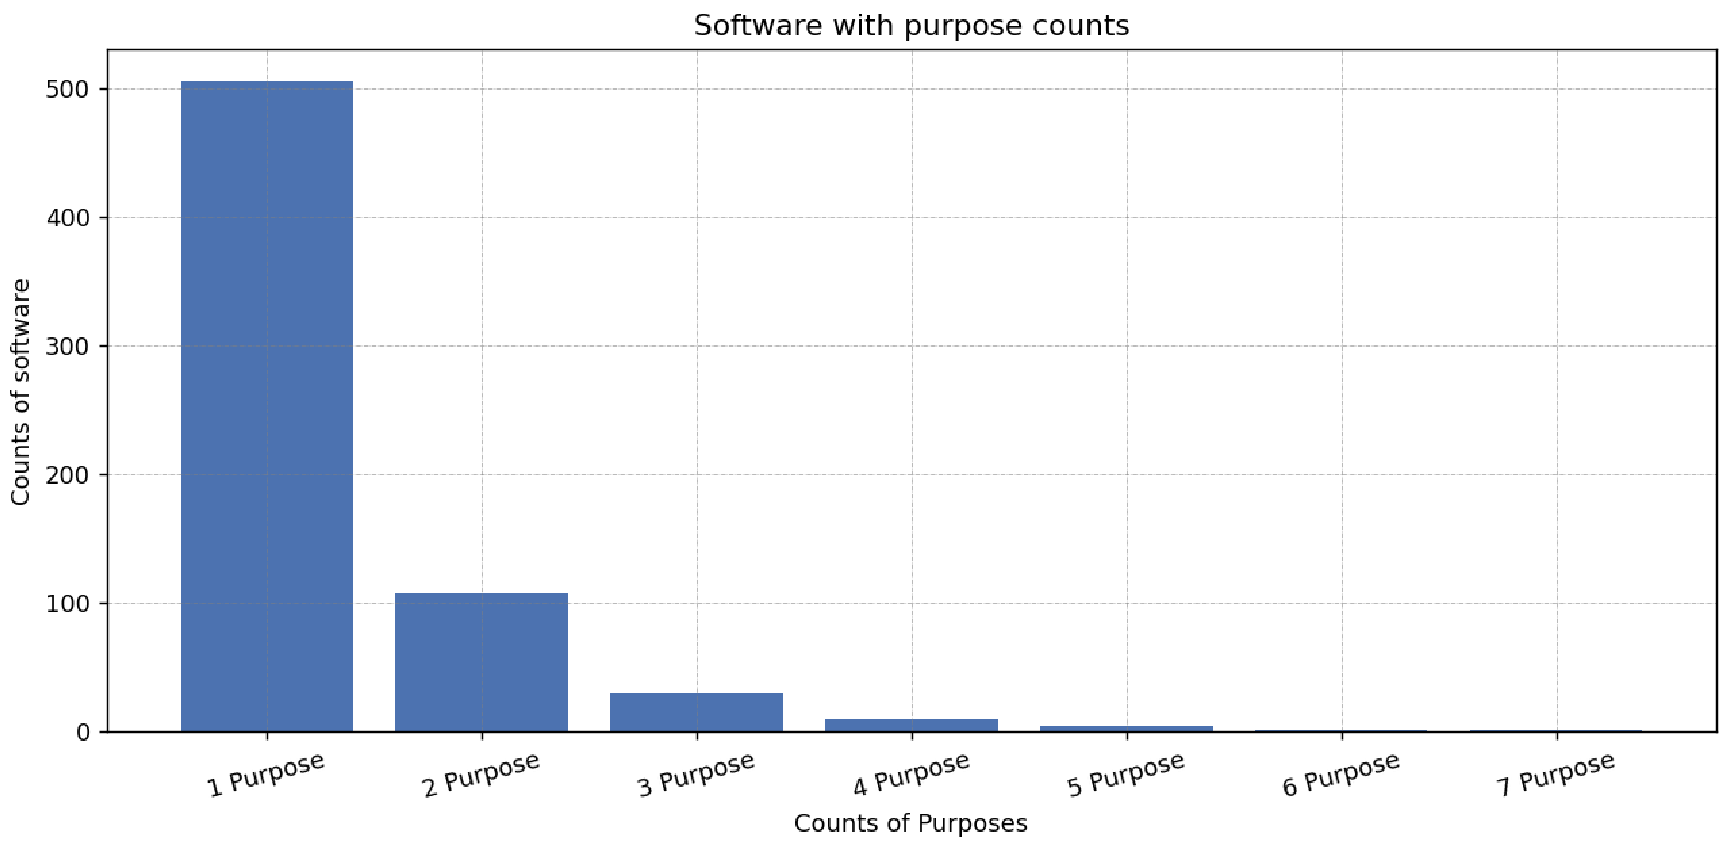
\includegraphics[width=.80\linewidth]{4.graphics/figures/ch_4/analysisresults/7.counts of software purpose}
	\label{fig:chapter03:subfloat:grafik1}
	\caption{Number of purposes a software is used for, most software tools in SoMeSci are used for just a specific purpose.}
\end{figure}



\section{Data Splitting and Optimization}
\label{subsec:dataset:preprocessing:Splitting}
After the data has been transformed into the IOB format, the data set, \ac{SoMeSci}, has been split into train, test and development set with  60, 20, 20 ratio respectively. To ensure the distribution  of enough samples of class labels, for all 8 types software usage purpose class labels, the data set has been iteratively split until each of software usage purpose class label lies within +/- 5\%  range for all train, test and development datasets. \\ 

Initially the iterative data splitting was carried out separately for PLoS methods and PubMed-full text. However, due to lack of enough class labels in PubMed-full text, especially for stimulation class, the iterative splitting did not converge. For this reason PLoS and PubMed articles have been combined to make the splitting converge. \\

The most optimal data split obtained from the iterative splitting is shown on the table 4.3 below, where there is still class imbalance for stimulation in the development data set. Finally, few articles from the test set have been manually moved into the development set to make the data split comply 100\% within +/- 5\%. \\

\begin{table}[ht]
	\centering
	\caption{The optimal data split for class labels before further manual balancing.}
	\begin{tabular*}{0.75\textwidth}{@{\extracolsep{\fill}}  c  c c  c c  }
		\hline
		Software Purpose & Train (\%)       & Dev.(\%)    & Test (\%)   & Total \\
		\hline 
		Analysis         & 890 (62\%)  & 263 (18\%)  & 283 (20\%)    & 1436 \\
		
		Data Collection  & 150 (61\%)  & 48 (19\%)   &  48 (20\%)    &  246\\
		
		Pre-processing   & 205 (61\%)  & 64 (19\%)   &  66 (20\%)    & 335 \\
		
		Modeling         & 141 (62\%)  & 35 (15\%)   &  51 (23\%)    & 227\\
		
		Programming      & 51 (64\%)   & 14 (17\%)   &  15(19\%)     &   80\\
		
		Stimulation      & 16 (57\%)   & 6 (21.5\%)  &   6 (21.5\%)  & 28\\
		
		Simulation       & 45 (63\%)   & 9 (13\%)    &   17 (20\%)   & 71 \\
		
		Visualization    & 70 (60\%)   & 27 (23\%)   &   20 (17\%)   & 117\\
		\hline
	\end{tabular*}
\end{table}%


Part of a python code for optimizing the data split has been listed on \emph{appendix D}. The notebook for data set splitting and optimization can be found on a git-hub repository\footnote{\url{https://github.com/BeTKH/SoMeNLP/tree/contxt2Sentcs_wo/bin}}. 


